%!TEX root = draft.tex
\section{The level-set method}

\indent The level-set method is a method to capture interfaces implicitely by constructing a function $\phi$, called the level-set function, that is negative on on side of the domain $\Omega^-$ and positive on the other side $\Omega^+$, thus defining the interface $\Gamma$ as the zero contour of $\phi$, $\Gamma = \{\mathbf{x} \vert \phi(\mathbf{x}=0\}$.\\

If infinitely many functions satisfy these requirements, the most natural and most convenient representation is a signed distance function to the interface. The level-set function is therefore reinitialized to a signed distance function at every time step by solving the reinitialization equation

\begin{equation} \label{eq::reinitialization}
\pd{\phi}{\tau} + \mathrm{sign}(\phi) \left( \lvert \phi \rvert - 1 \right) = 0,
\end{equation}

where $\tau$ is a fictitious time. The discretization and implementation of this procedure will be discussed later in section \ref{section::reinitialization}. Geometrical quantities such as the normal to the interface and the local curvature can be computed straightforwardly from the level-set function as

\begin{equation*}
\mathbf{n} = \frac{\nabla \phi}{\lvert \nabla \phi \rvert},
\end{equation*}

where it should be noted that $\lvert \nabla \phi \rvert = 1$ when the level-set function is reinitialized, and

\begin{equation*}
\kappa = \nabla \cdot \mathbf{n} =  \nabla \cdot \left( \frac{\nabla \phi}{\lvert \nabla \phi \rvert} \right).
\end{equation*}


\section{The \texttt{p4est} library}

The work we present relies on the parallel octree library \texttt{p4est} \cite{burstedded:2011:p4est}. It is scalable implementation of the general octree structure in a massively parallel mpi environment. We limit our presentation of \texttt{p4est} to the relevant information for our application, for more details the reader is invited to read the original article \cite{burstedded:2011:p4est}.

The \texttt{p4est} library provides the geometrical information for the leaves of an octree which includes the neighboring information for the leaves (called quadrants in the original article) of the tree, a layer of ghost quadrants and ghost vertices for each process, the coarsening and refining procedures, and encapsulates the communication between processes. However, it does not provide the vertical structure of the octrees. If it is generally unnecessary, it is a desirable feature for a finite differences based code as it speeds up the access to arbitrary quadrants information dramatically. Thus, we choose to reconstruct the local vertical structure of the octree on every processes. Note that given the local and ghost layer information, this is an entirely local procedure and no communication is needed.

In addition to the owned and ghost categories, we choose to group the vertices in \textit{local} and \textit{layer} sets. We define the layer vertices as the vertices that are part of another process's ghost layer and the local vertices as the vertices that are not part of any other process's ghost layer. Figure \ref{fig::local_layer_vertices} gives a graphical representation of a boundary between two processes and the classification of the various quadrants and vertices. The idea behind this sorting is that layer vertices are needed by other processes for finite difference calculations and therefore require to be synchronized while the local vertices are used only by the process they belong to. We make use of this classification to implement scalable algorithms for the level-set method, as explained in the following sections.

\begin{figure}[ht!]
\begin{center}
\includegraphics[width=.4\textwidth]{pictures/layer_nodes.pdf}
\caption{Illustration of a possible layout at the interface between two processes. The red quarants and the orange and purples vertices belong to process 1 while the green quadrants and the green and black vertices belong to process 2. The green G denotes the ghost quadrants for process 2, the green dots are the ghost vertices for process 1, and the purple dots correspond to layer vertices for process 1 (and therefore ghost vertices for process 2).} \label{fig::local_layer_vertices}
\end{center}
\end{figure}